\documentclass[tikz,border=5mm]{standalone}
\usepackage{tikz}
\usetikzlibrary{arrows.meta,positioning}
\begin{document}
% Grafcet : A1_POST
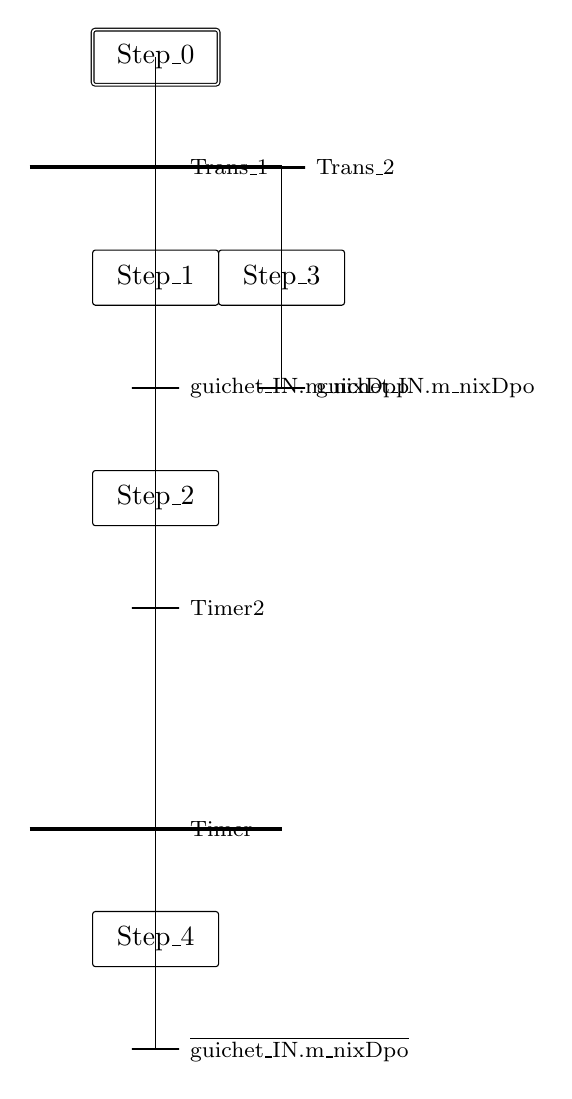
\begin{tikzpicture}[
  sfcstep/.style  = {draw, rounded corners=1pt, minimum width=16mm, minimum height=7mm, inner sep=1pt},
  sfcinit/.style  = {draw, double, rounded corners=1pt, minimum width=16mm, minimum height=7mm, inner sep=1pt},
  sfctrans/.style = {draw, line width=0.8pt, minimum width=6mm, minimum height=0pt, inner sep=0pt},
  sfcbranch/.style= {line width=1.4pt},
  sfclink/.style  = {->, >=Stealth, line width=0.8pt},
  x=16mm, y=-14mm,
]

  \node[sfcinit] (s65537) at (4.00,1.00) {Step\_0};
  \node[sfcstep] (s65538) at (4.00,3.00) {Step\_1};
  \node[sfcstep] (s65539) at (4.00,5.00) {Step\_2};
  \node[sfcstep] (s65540) at (5.00,3.00) {Step\_3};
  \node[sfcstep] (s65541) at (4.00,9.00) {Step\_4};
  \node[sfctrans,label={right:\footnotesize Trans\_1}] (t0) at (4.00,2.00) {};
  \node[sfctrans,label={right:\footnotesize guichet\_IN.m\_nixDpp}] (t1) at (4.00,4.00) {};
  \node[sfctrans,label={right:\footnotesize Timer}] (t2) at (4.00,8.00) {};
  \node[sfctrans,label={right:\footnotesize Trans\_2}] (t3) at (5.00,2.00) {};
  \node[sfctrans,label={right:\footnotesize guichet\_IN.m\_nixDpo}] (t4) at (5.00,4.00) {};
  \node[sfctrans,label={right:\footnotesize $\overline{\mbox{guichet\_IN.m\_nixDpo}}$}] (t5) at (4.00,10.00) {};
  \node[sfctrans,label={right:\footnotesize Timer2}] (t6) at (4.00,6.00) {};
  \draw[sfcbranch] (3.00,2.00) -- (5.00,2.00);
  \draw[sfcbranch] (3.00,8.00) -- (5.00,8.00);
  \draw (4.00,1.00) -- (4.00,2.00);
  \draw (4.00,2.00) -- (4.00,3.00);
  \draw (4.00,3.00) -- (4.00,4.00);
  \draw (4.00,4.00) -- (4.00,5.00);
  \draw (4.00,5.00) -- (4.00,6.00);
  \draw (4.00,6.00) -- (4.00,8.00);
  \draw (4.00,8.00) -- (4.00,9.00);
  \draw (4.00,9.00) -- (4.00,10.00);
  \draw (5.00,2.00) -- (5.00,3.00);
  \draw (5.00,3.00) -- (5.00,4.00);
\end{tikzpicture}
\end{document}
